\documentclass[linenumbers,twocolumn]{aastex631}
\usepackage[utf8]{inputenc}
\usepackage{natbib}
\setcitestyle{round}
\usepackage{amsmath,amssymb}
\usepackage{afterpage}
\usepackage{xcolor}
\usepackage[caption=false]{subfig}
\usepackage{soul}
\usepackage{enumitem}
\usepackage{xcolor}
\usepackage{graphicx}
\usepackage{listings}
\usepackage{listings}
\lstset{
    basicstyle=\footnotesize\ttfamily,
    breaklines=true,
    xleftmargin=0.1\linewidth,
    xrightmargin=0.1\linewidth
}

\newcommand{\hi}{{\rm H\,{\small I}}}
\newcommand{\kms}{\ensuremath{{\rm km~s^{-1}}}}
\newcommand{\persc}{\ensuremath{{\rm cm^{-2}}}}
\newcommand{\msun}{\ensuremath{M_{\odot}}}



\begin{document}

\title{Astron 465 - Optical Lab 2 - Photometry of Star Clusters}



\author[0009-0002-9802-0511]{Riya Kore}
\affiliation{University of Wisconsin--Madison, Department of Astronomy, 475 N Charter St, Madison, WI 53703, USA}

\section{Introduction} \label{sec:introduction}

\subsection{Overview of Photometry and its Importance}

Photometry, the precise measurement of an object's brightness, serves as a fundamental tool in observational astrophysics. By quantifying the light emitted or reflected by celestial objects, astronomers can infer key physical properties, such as temperature, luminosity, chemical composition, and distance. This lab focuses on the photometric analysis of star clusters, specifically the open cluster NGC 1528, to explore its stellar population and evolutionary characteristics. This lab involves reducing raw astronomical data, calibrating images using bias and flat-field corrections, and analyzing the reduced data to construct color-magnitude diagrams (CMDs). These diagrams are essential observational counterparts to the Hertzsprung-Russell Diagram (HRD) and play a crucial role in understanding stellar evolution. \\

Star clusters are among the most significant objects in astrophysics, offering valuable insights into stellar evolution and the structure of our galaxy. They are typically categorized into three types: globular clusters, open clusters, and stellar associations. Globular clusters are dense, spherical systems composed of hundreds of thousands of old, metal-poor stars located in the galactic halo. Open clusters, such as NGC 1528, are loosely bound groups of younger stars found within the galactic disk. In contrast, stellar associations contain even fewer stars and are only weakly gravitationally bound. Studying open clusters provides a unique opportunity to investigate the properties and evolutionary states of stars formed under similar initial conditions. The relatively sparse population of open clusters like NGC 1528 makes them particularly suitable for photometric analysis.

\subsection{The Hertzsprung-Russell Diagram and Color-Magnitude Diagrams}

The Hertzsprung-Russell Diagram (HRD) is a cornerstone of stellar astrophysics, illustrating the relationship between a star's luminosity and its surface temperature. The observational equivalent, the Color-Magnitude Diagram (CMD), plots a star's apparent magnitude against its color index, such as (B-V) or (g-i). CMDs are crucial tools for investigating the evolutionary stages of stars, including the main sequence, red giant branch, and white dwarf cooling sequence. Additionally, CMDs allow astronomers to estimate key properties of star clusters, such as age, metallicity, and distance, by comparing observational data to theoretical isochrones. In this lab, the CMD constructed for NGC 1528 serves as a tool to examine the cluster's stellar population and evolutionary status.

\subsection{Photometric Calibration and Data Reduction}

Accurate photometric measurements require meticulous calibration and data reduction. Raw CCD images often contain artifacts, such as electronic noise, uneven pixel sensitivity, and detector response variations, which must be corrected before analysis. The first step in this process involves bias correction, which removes the baseline electronic noise intrinsic to the CCD detector. This is followed by flat-fielding, where flat-field images correct for pixel-to-pixel sensitivity variations, ensuring uniform detector response across all pixels. The calibration process involves subtracting the master bias image and dividing by the master flat-field image to produce scientifically valid data. These steps are essential for minimizing systematic errors and ensuring precise photometric measurements.

\subsection{NGC 1528 and Observational Details}

In this lab, the focus is on the photometric analysis of NGC 1528, an open cluster known for its relatively sparse but well-defined stellar population. Observations were conducted using a CCD telescope connected to a Raspberry Pi, with data collected in multiple photometric bands, including g, r, and i. The choice of these bands allows for robust color analysis, which is essential for CMD construction. The data acquisition process included capturing bias frames to measure electronic noise, flat fields to correct for detector non-uniformities, and science images to capture the light emitted by the cluster's stars. These calibrated images form the foundation of the lab's photometric analysis.

\subsection{Lab Objectives and Computational Approach}

The objectives of this lab are twofold. First, the lab aims to develop a thorough understanding of photometric calibration techniques through hands-on data reduction. Second, it seeks to use the reduced data to perform photometric measurements and construct CMDs for NGC 1528. Computational tools, including Python-based libraries such as Astropy and Photutils, are employed for data reduction, source detection, and photometric measurements. These tools streamline the analysis process and allow for efficient handling of large datasets, making them indispensable for this lab. \\

This lab emphasizes the critical role of systematic calibration and data processing in astrophysics. By integrating theoretical knowledge with practical techniques, the study of NGC 1528 provides insights into stellar evolution and galactic structure. The lab serves as a framework for understanding photometric methods that can be extended to other star clusters and celestial phenomena, contributing to a deeper understanding of the universe.

\section{Observations} \label{sec:observations}

In this lab, observations were conducted to enable accurate photometric analysis of the star cluster NGC 1528, building upon the work from the first part of this lab. The observational process involved gathering bias images, flat fields, and science images in multiple photometric bands using a CCD telescope controlled through a Raspberry Pi setup with Astroberry and CCDeil software. These observations are central to constructing color-magnitude diagrams (CMDs) for understanding the properties of the star cluster.

\subsection{Data Acquisition Setup}

The data acquisition process was facilitated by a CCD telescope equipped with a multi-band filter wheel. Remote control of the telescope functions and CCD settings was achieved using Astroberry and CCDeil software. For this phase of the lab, additional emphasis was placed on monitoring the CCD temperature to ensure consistency across multiple observation sessions. Adjustments to exposure time and filter selection were optimized to maximize signal-to-noise ratios in the g, r, and i bands, which are critical for precise photometric analysis. Each image was carefully labeled and organized, ensuring seamless integration into the calibration and reduction pipeline. \\\\

\subsection{Bias Images Collection}

Bias images were collected to measure the baseline electronic noise inherent to the CCD detector. For consistency with the earlier lab, six bias frames were obtained under identical conditions, using zero exposure time and keeping the telescope shutter closed. These frames were averaged to produce a master bias image, which was later applied to all science images to correct for electronic noise. The uniformity and reliability of the bias images were verified by examining pixel intensity distributions, confirming the absence of anomalies or outliers.

\begin{figure}[h] 
    \centering 
    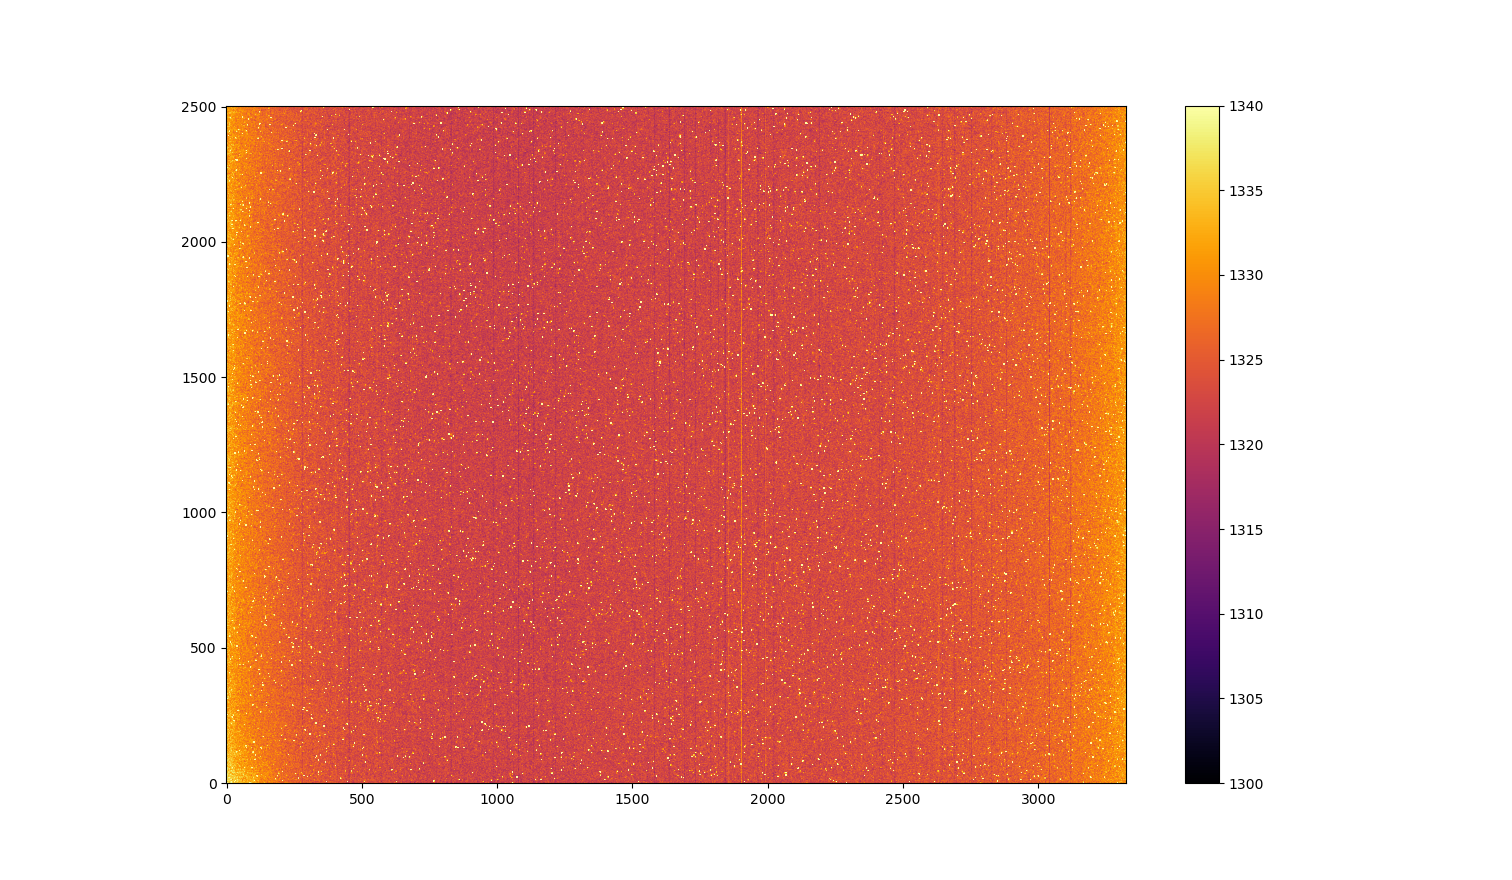
\includegraphics[width=0.9\linewidth]{bias_raw.png} 
    \caption{Bias image showing electronic noise patterns across the CCD, displayed with a range set to mean ± standard deviation.} 
    \label{fig:one_bias} 
\end{figure}

\begin{figure}[h]
    \centering
    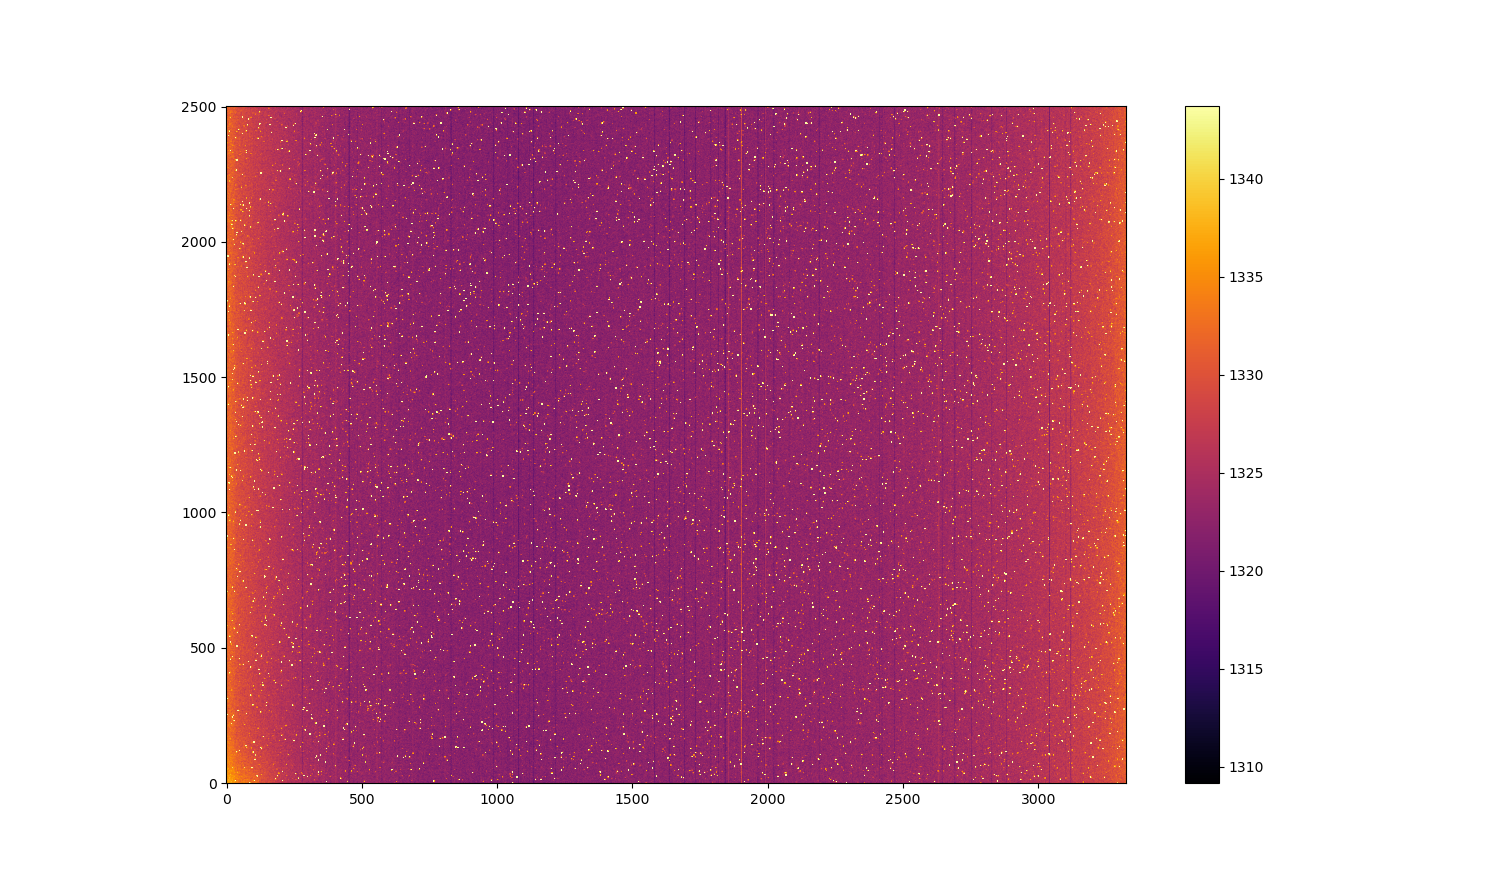
\includegraphics[width=0.9\linewidth]{master_bias.png}
    \caption{Master bias image created by averaging multiple bias frames, showing the baseline electronic noise across the CCD.}
    \label{fig:master_bias}
\end{figure}

\subsection{Flat Field Images Collection}

Flat field images were obtained to correct for pixel sensitivity variations across the CCD detector. Images were taken in the g, r, and i bands by exposing the CCD to a uniformly illuminated field. For each band, five flat field frames were captured, ensuring sufficient data to account for pixel-to-pixel variations. These frames were normalized and combined to create master flat field images for each band, which were subsequently used to calibrate the science images. The uniformity of illumination and the effectiveness of the flat field corrections were evaluated by examining pixel intensity histograms and spatial gradients across the images.

\begin{figure}[h]
    \centering
    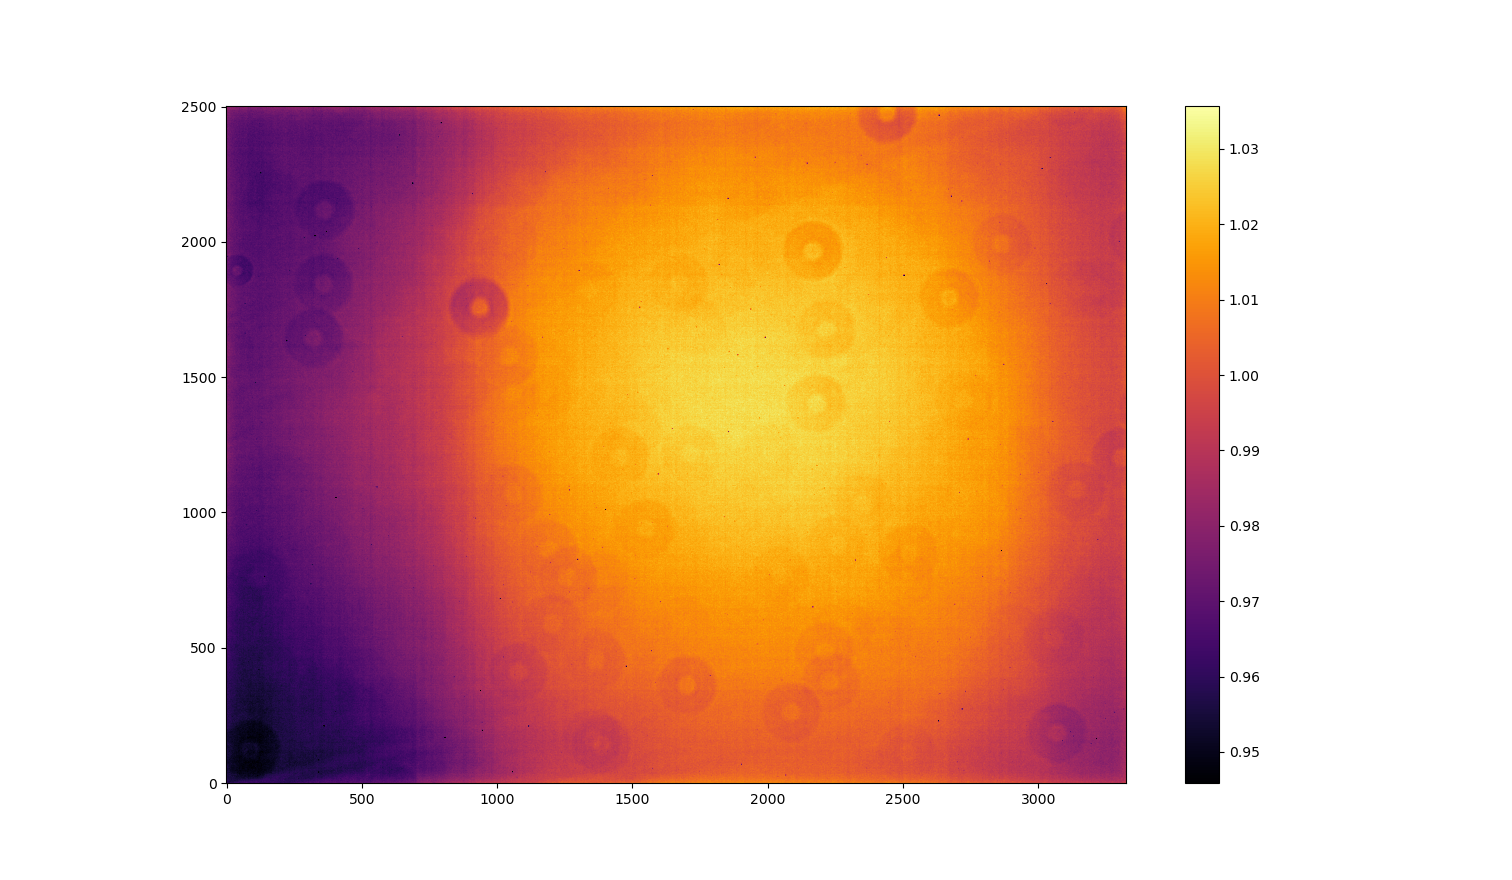
\includegraphics[width=0.9\linewidth]{master_flat_g.png}
    \caption{Master flat field image for the g-band, used to correct pixel sensitivity variations in the science images.}
    \label{fig:master_flat_g}
\end{figure}

\begin{figure}[h]
    \centering
    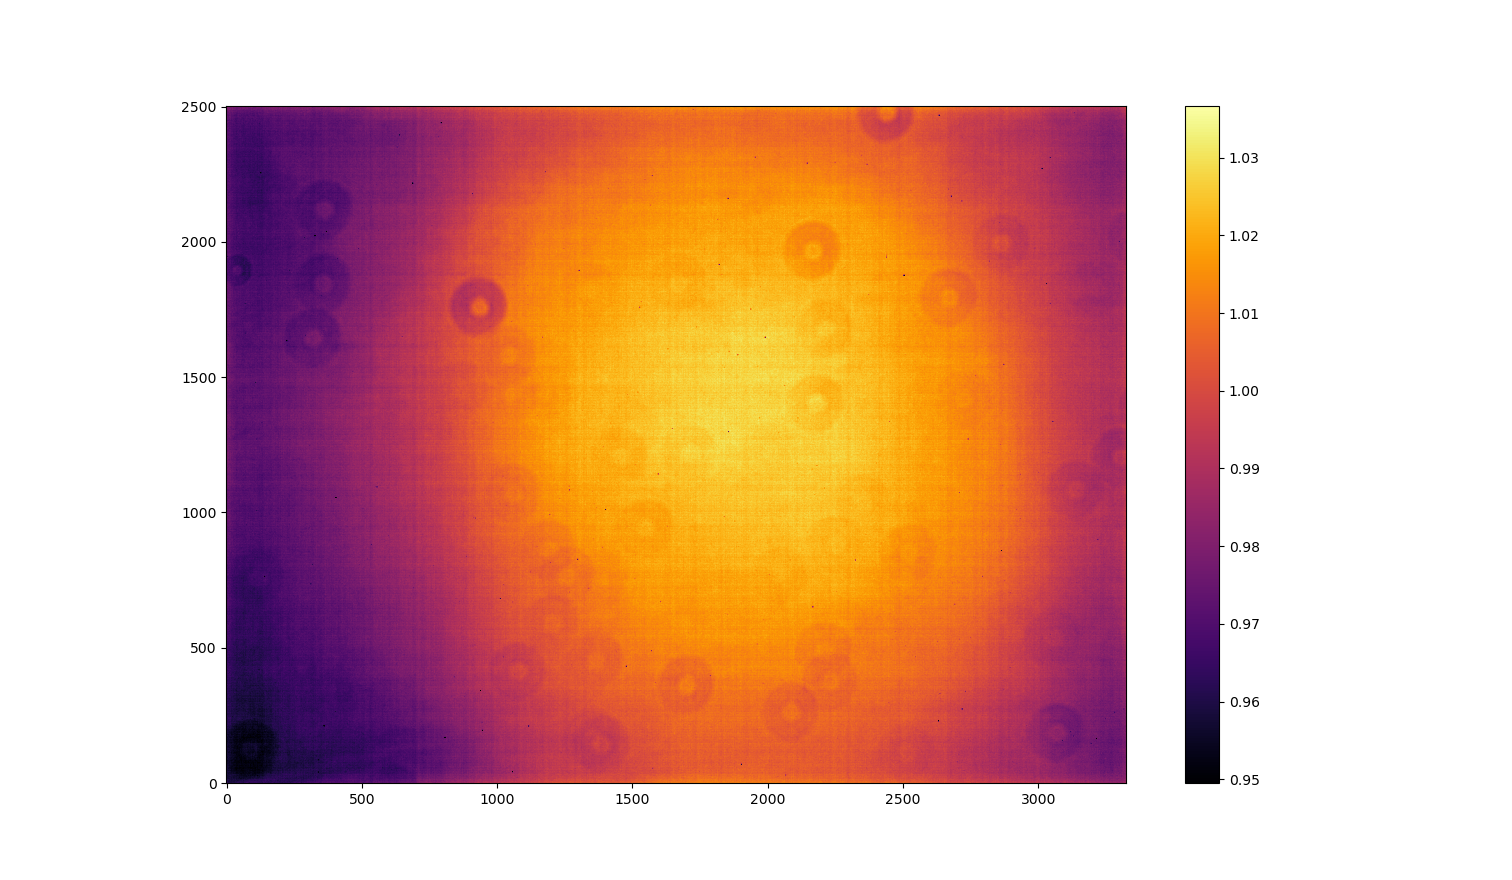
\includegraphics[width=0.9\linewidth]{master_flat_r.png}
    \caption{Master flat field image for the r-band, used to correct pixel sensitivity variations in the science images.}
    \label{fig:master_flat_r}
\end{figure}

\begin{figure}[h]
    \centering
    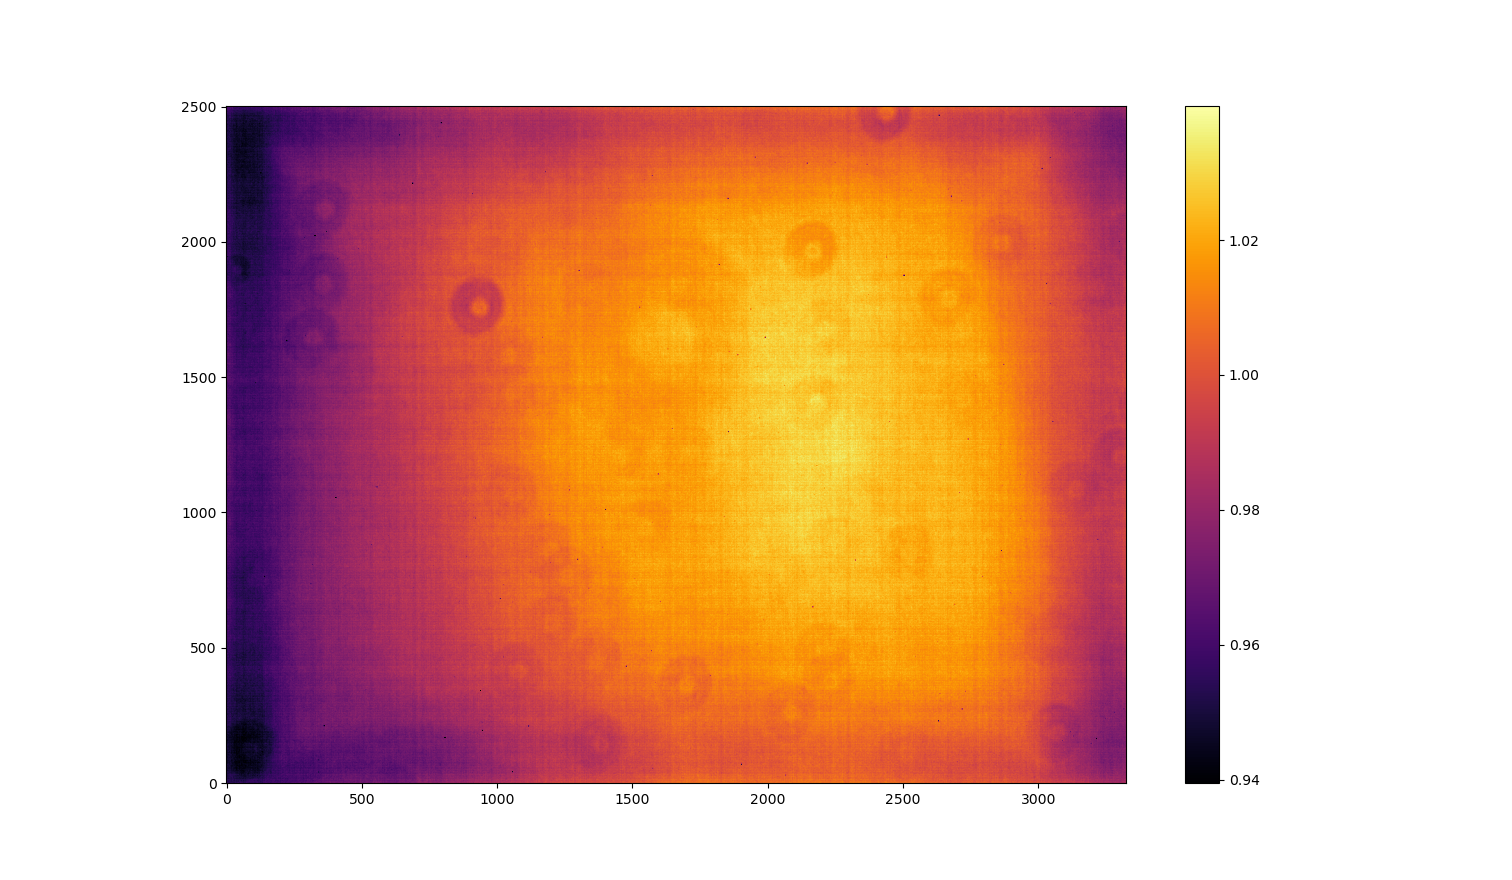
\includegraphics[width=0.9\linewidth]{master_flat_i.png}
    \caption{Master flat field image for the i-band, used to correct pixel sensitivity variations in the science images.}
    \label{fig:master_flat_i}
\end{figure}

\subsection{Science Images of NGC 1528}

To facilitate the construction of a CMD for NGC 1528, science images were captured in the g, r, and i bands. Each band included 5-6 frames, providing sufficient redundancy to mitigate noise and artifacts during the reduction process. The science images displayed a clear view of the star cluster, highlighting its stellar population against the background sky. These images serve as the primary dataset for photometric measurements, enabling the extraction of brightness and color indices for individual stars. Examples of these science images, calibrated and ready for analysis, are shown in Figures~\ref{fig:reduced_g}, \ref{fig:reduced_r}, and \ref{fig:reduced_i}.

\begin{figure}[h]
    \centering
    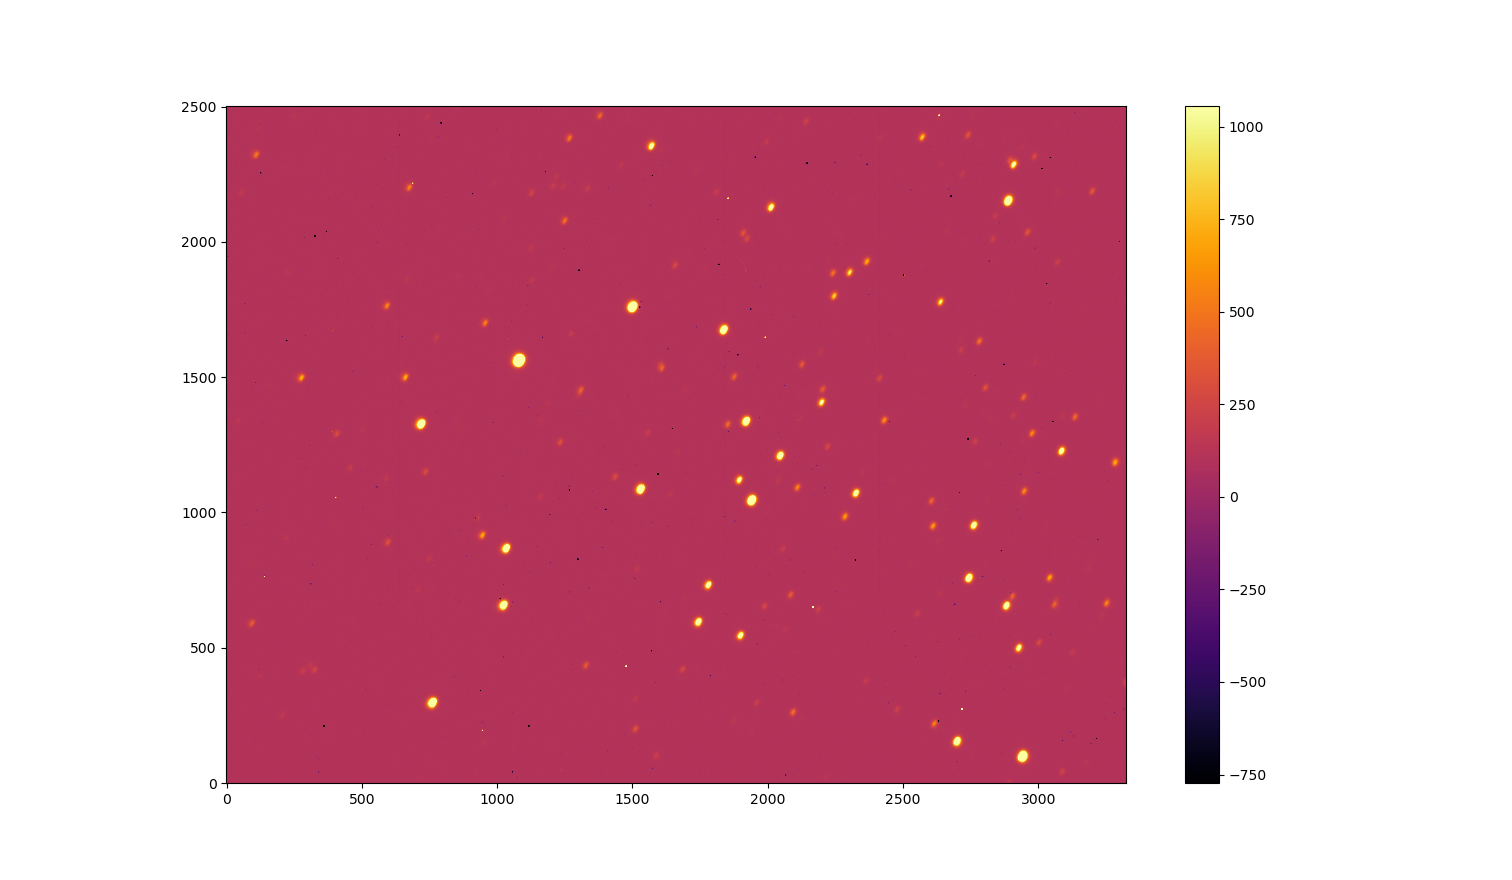
\includegraphics[width=0.9\linewidth]{reduced_science_g.png}
    \caption{Reduced science image in the g-band after bias subtraction and flat field correction.}
    \label{fig:reduced_g}
\end{figure}

\begin{figure}[h]
    \centering
    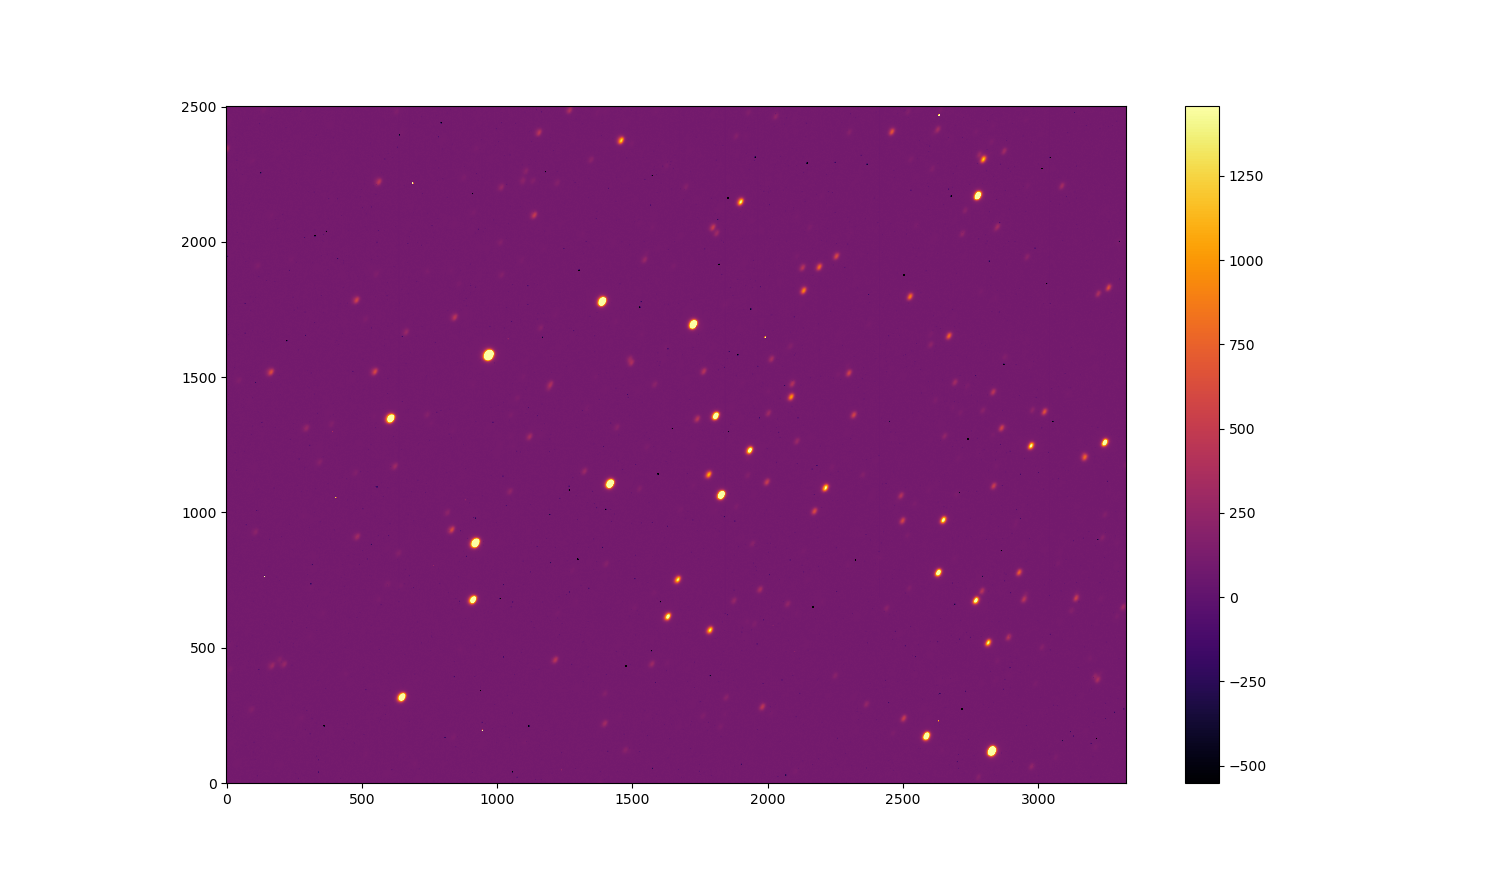
\includegraphics[width=0.9\linewidth]{reduced_science_r.png}
    \caption{Reduced science image in the r-band after bias subtraction and flat field correction.}
    \label{fig:reduced_r}
\end{figure}

\begin{figure}[h]
    \centering
    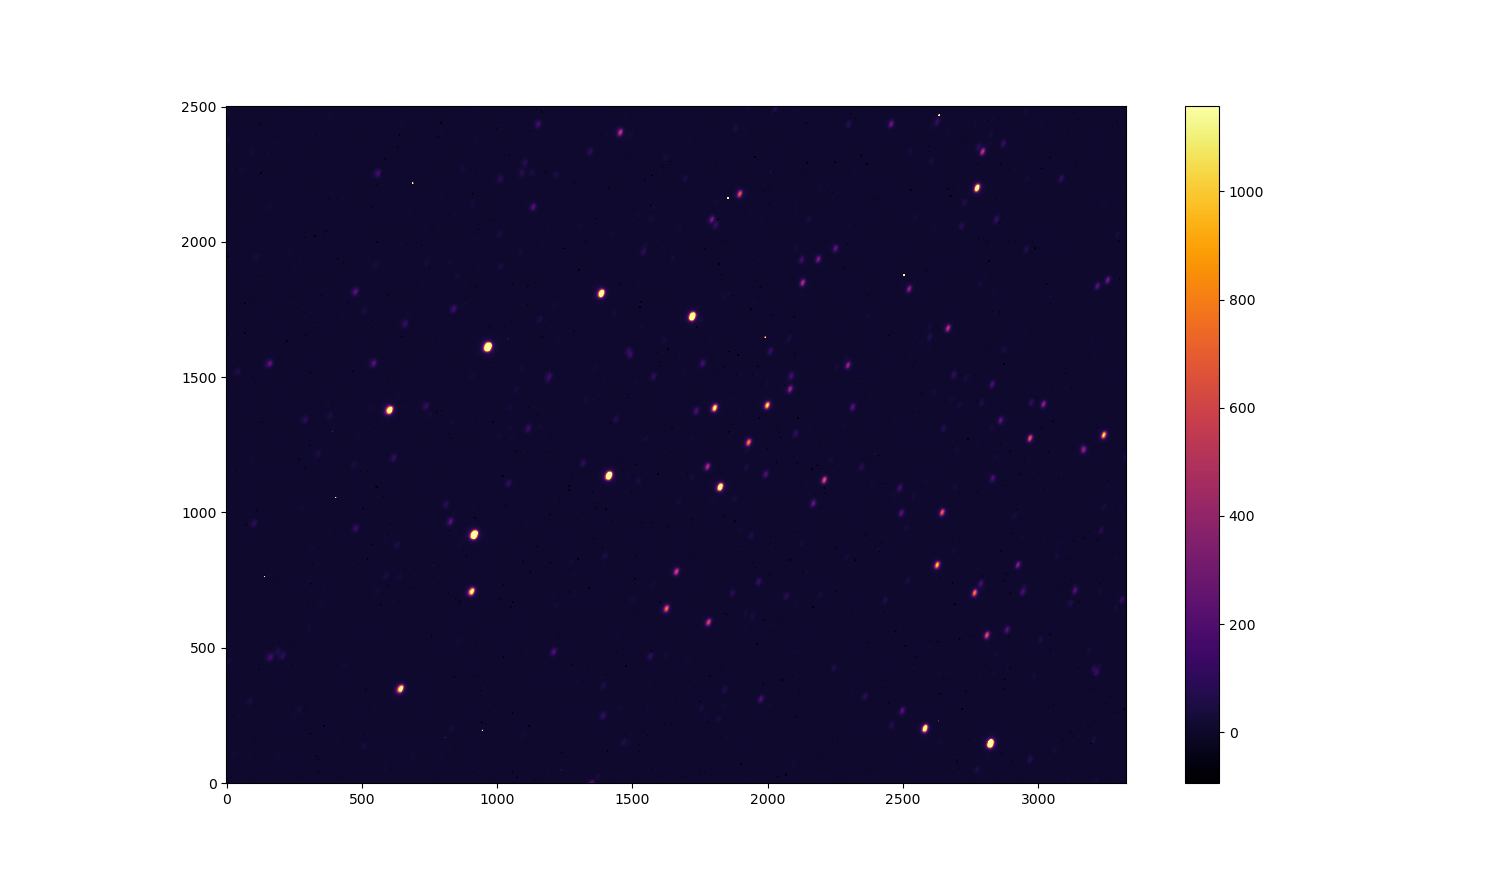
\includegraphics[width=0.9\linewidth]{reduced_science_i.png}
    \caption{Reduced science image in the i-band after bias subtraction and flat field correction.}
    \label{fig:reduced_i}
\end{figure}

\subsection{Challenges and Refinements}

During this phase of the lab, the telescope's tracking system was carefully calibrated to prevent alignment errors encountered in the earlier session. Although no major issues arose, additional steps were taken to validate the quality of the calibration images. For instance, flat field images were re-examined to confirm uniformity across all bands, and additional bias frames were captured to ensure consistency with previous results. The telescope’s positioning system was also recalibrated to avoid potential tracking errors during longer exposure sessions.

\section{Data analysis} \label{sec:results}

This section details the steps undertaken for reducing, analyzing, and interpreting the observational data collected during the photometric study of the star cluster NGC 1528. It covers the calibration of science images, extraction of photometric information, and alignment of data across different filters to prepare for further astrophysical analyses.

\subsection{Calibration of Science Images}

The first step in the data analysis invoked calibrating the raw science images using bias and flat-field corrections. A \texttt{Reduce} class was implemented to facilitate this process programmatically. Bias correction was performed by creating a master bias frame. The process began by loading all individual bias images using the \texttt{astropy.io.fits} module, followed by stacking these images into a 3D array. A median operation was applied along the stacking axis to produce the master bias frame, which effectively removed electronic noise intrinsic to the CCD detector. The master bias was saved as a FITS file for further use in the calibration pipeline. Flat-field correction aimed to normalize pixel-to-pixel sensitivity variations in the CCD. Separate sets of flat-field images for the g-, r-, and i-band filters were processed. Each image was bias-subtracted and normalized to its mean intensity to ensure consistent brightness calibration across the CCD. The normalized images were then stacked, and a median operation was applied to generate master flat-field frames for each filter. These master flat fields were used to correct science images by dividing the pixel values of each science frame by the corresponding master flat field, effectively eliminating sensitivity and illumination variations. The calibrated science images were subsequently saved for analysis. This is the pyhton code for the entire process: \\\\

\begin{lstlisting}[language=Python]
class Reduce:
    def make_master_bias(bias_directory_path, mean = False):
        bias_files_list = glob.glob(bias_directory_path)
        bias_images_stack = []
        for filename in bias_files_list:
            image = fits.open(filename)[0].data.astype(float)
            bias_images_stack.append(image)
        bias_stack = np.array(bias_images_stack)
        if mean == True:
            master_bias = np.mean(bias_stack, axis = 0)
            fits.PrimaryHDU(data = master_bias).writeto("master_bias_mean.fits", overwrite = True)
            return master_bias
        if mean == False:
            master_bias = np.median(bias_stack, axis = 0)
            fits.PrimaryHDU(data = master_bias).writeto("master_bias_median.fits", overwrite = True)
            return master_bias

    def make_master_flat_field(flat_field_directory_path, master_bias, g = True, i = True):
        flats_files_list = glob.glob(flat_field_directory_path)
        flats_images_stack = []
        for filename in flats_files_list:
            image = fits.open(filename)[0].data.astype(float)
            image = image - master_bias
            mean_level = np.mean(image)
            image = image / mean_level
            flats_images_stack.append(image)
        flats_stack = np.array(flats_images_stack)
        master_flat = np.median(flats_stack, axis = 0)
        # g filter
        if g == True and i == False:
            fits.PrimaryHDU(data = master_flat).writeto("masterflat_g.fits", overwrite = True)
        # r filter
        if g == False and i == False:
            fits.PrimaryHDU(data = master_flat).writeto("masterflat_r.fits", overwrite = True)
        # i filter
        if g == False and i == True:
            fits.PrimaryHDU(data = master_flat).writeto("masterflat_i.fits", overwrite = True)
        return master_flat

    def reduce_science_image(science_image_path, master_bias, master_flat):
        image = fits.open(science_image_path)[0].data.astype(float)
        image = image - master_bias
        image = image / master_flat
        return image
\end{lstlisting}

\subsection{Background Estimation and Source Detection}

The next phase of the analysis focused on extracting photometric information from the science images. The \texttt{Extract} class was developed to perform background subtraction, source detection, and flux estimation. Background subtraction was accomplished using the \texttt{sigma\_clipped\_stats} function from the \texttt{astropy.stats} package, which computes robust statistical metrics while excluding outliers caused by sources or cosmic rays. The computed background was subtracted from the science image to produce a background-subtracted frame, enabling precise detection of astrophysical sources.

Source detection was carried out using the \texttt{DAOStarFinder} algorithm, which identifies sources by searching for local maxima above a threshold defined as multiples of the background noise standard deviation. The threshold used here is 5$\sigma$. The algorithm also computes key properties of detected sources, such as centroid positions, sharpness, and flux. These properties were stored in a table for further processing. The source detection step was validated by visually inspecting scatter plots of detected sources which you can see in the figures ~\ref{fig:sources_g}, \ref{fig:sources_r}, and \ref{fig:sources_i}. This is the python code used:

\begin{lstlisting}[language=Python]
class Extract:

    def estimate_background(image_data):
        # this is using the astropy.stats package
        mean, background, std = sigma_clipped_stats(image_data, sigma=3.0)
        background_subtracted_image = image_data - background
        return background_subtracted_image, std, background

    def detect_source(background_subtracted_image, std, threshold):
        daofind = DAOStarFinder(fwhm=3.0, threshold=threshold*std)
        sources = daofind(background_subtracted_image)
        for col in sources.colnames:
            if col not in ('id', 'npix'):
                sources[col].info.format = '%.2f'
        sources = sources.to_pandas()
        return sources
\end{lstlisting}

\begin{figure}[h]
    \centering
    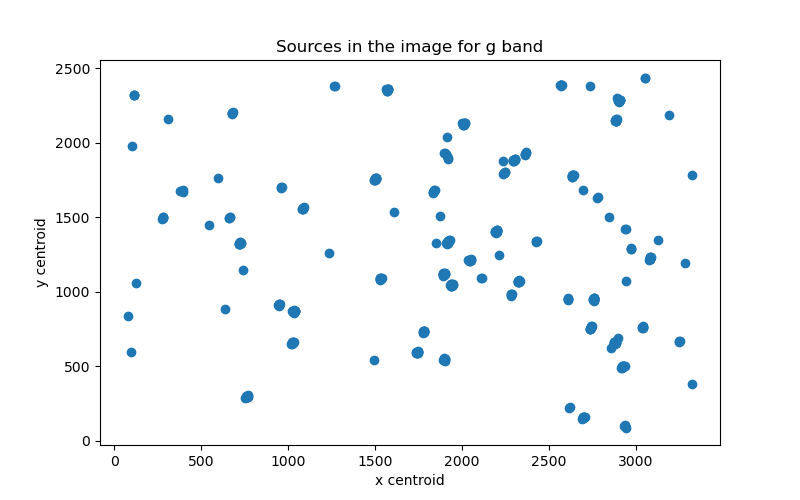
\includegraphics[width=0.9\linewidth]{sources_g.png}
    \caption{Visual of the sources in the reduced science image for the g band with a threshold of 5$\sigma$.}
    \label{fig:sources_g}
\end{figure}

\begin{figure}[h]
    \centering
    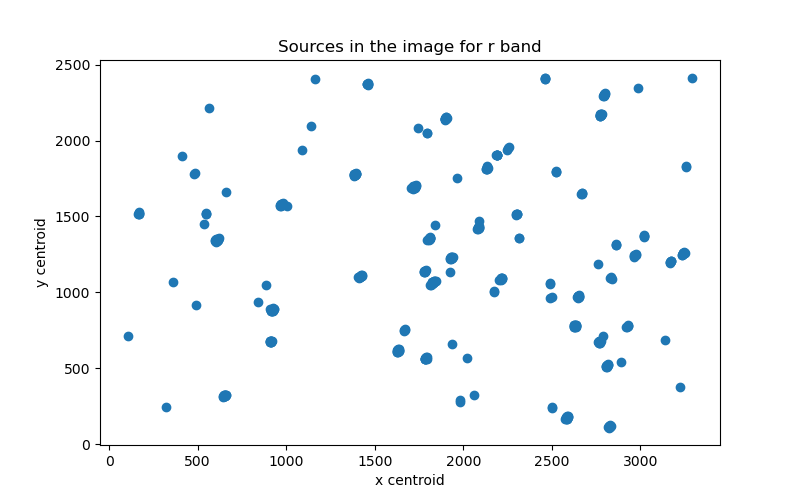
\includegraphics[width=0.9\linewidth]{sources_r.png}
    \caption{Visual of the sources in the reduced science image for the r band with a threshold of 5$\sigma$.}
    \label{fig:sources_r}
\end{figure}

\begin{figure}[h]
    \centering
    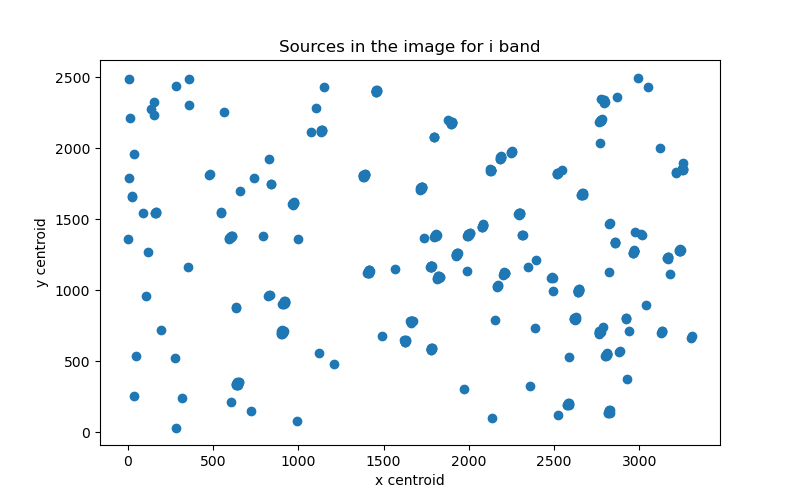
\includegraphics[width=0.9\linewidth]{sources_i.png}
    \caption{Visual of the sources in the reduced science image for the i band with a threshold of 5$\sigma$}
    \label{fig:sources_i}
\end{figure}

\subsection{Flux Estimation and Photometric Calibration}

Fluxes of detected sources were estimated through aperture photometry. Circular apertures with a fixed radius of 4 pixels were placed around each source centroid, and the total flux within the aperture was computed using the \texttt{aperture\_photometry} function from the \texttt{photutils} package. Magnitudes were calculated using the standard relation.

\begin{equation}
    \text{mag} = -2.5  \ log_{10}(\text{aperture sum})
\end{equation}
To account for statistical uncertainties in flux measurements, flux errors were computed based on the CCD equation incorporating read noise, background noise, and aperture size. Here is the python code used for this process:

\begin{lstlisting}[language=Python]
class Extract:
    def estimate_source_fluxes(sources, background_subtracted_image):
        # provide source positions in the format the aperture tool requires
        positions = [ (sources.iloc[i]['xcentroid'], sources.iloc[i]['ycentroid']) for i in range(len(sources))]
        # define an aperture circular with radius equal to 4 pixels
        apertures = CircularAperture(positions, r = 4.0)
        # use aperture photometry tool
        photometry_table = aperture_photometry(background_subtracted_image, apertures)
        photometry_table['aperture_sum'].info.format = '%.8g'
        # source flux in  magnitudes = 2.5 log_10 (aperture sum)
        sources['aperture_sum'] = photometry_table['aperture_sum']
        sources['mag'] = -2.5*np.log10(sources['aperture_sum'])
        # print(sources['aperture_sum'])
        
        return sources

    def get_flux_uncertainties(sources, background):
        R = 9.904
        gain = 1.0
        npix = np.pi * 4**2
        sources['flux_err'] = np.sqrt(gain * sources['aperture_sum'] + npix*(gain*background + R**2)) / gain
        # converting it to a numpy array from an astropy table column
        return sources
\end{lstlisting}

\begin{figure}[h]
    \centering
    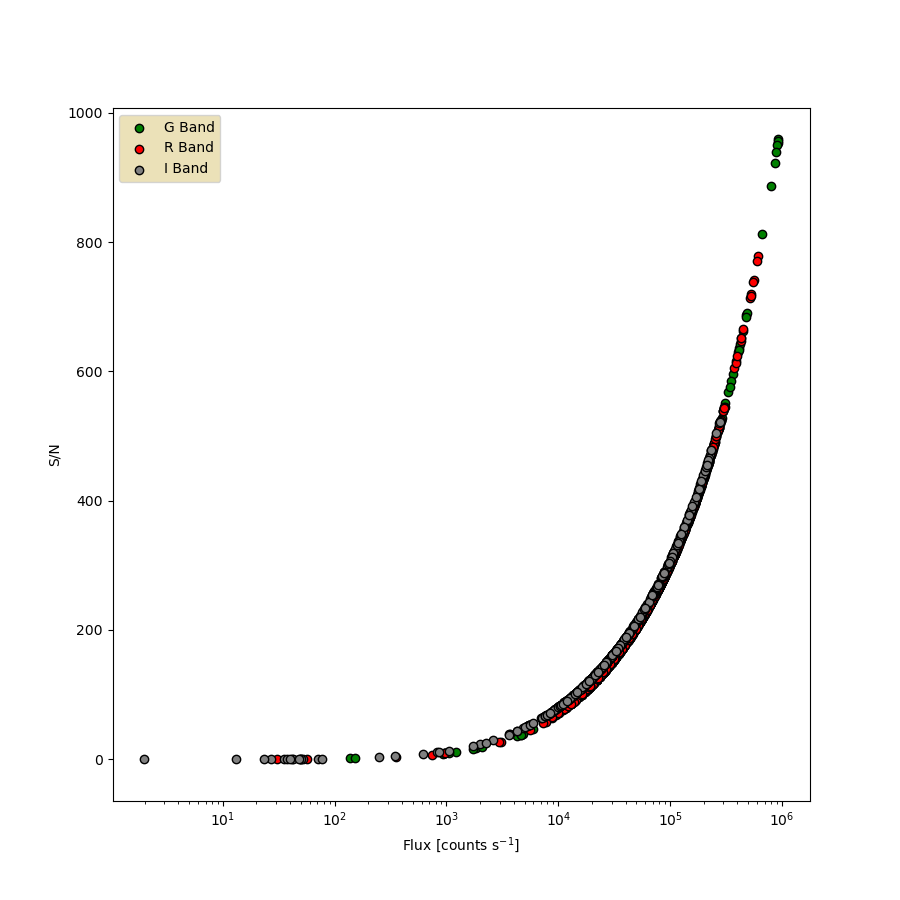
\includegraphics[width=0.9\linewidth]{flux_uncertainties.png}
    \caption{Uncertainties for the sources in the g, i, r bands.}
    \label{fig:uncertainties}
\end{figure}

Photometric calibration was performed by cross-matching the detected sources with a reference catalog from the Pan-STARRS database. The matched sources provided instrumental and catalog magnitudes for the same stars, enabling the computation of zero-point offsets for the g-, r-, and i-bands. These zero-points were applied to adjust the instrumental magnitudes of all detected sources, ensuring consistency with the standard photometric system. The zero points values we got are:
\begin{itemize}
    \item Zero Point for g-band: 23.817652348729098
    \item Zero Point for r-band: 23.420702182105735
    \item Zero Point for i-band: 22.59451412824947
\end{itemize}

This is the python code used to find the zero point values:

\begin{lstlisting}[language=Python]
import numpy as np
from astroquery.vizier import Vizier
from astropy.coordinates import SkyCoord
from astropy import units as u

ngc1528_center = SkyCoord(ra=65.71, dec=51.21,unit='deg')
search_radius = 2 * u.deg

Vizier.ROW_LIMIT = -1
catalog = Vizier.query_region(ngc1528_center, radius=search_radius, catalog="II/349/ps1")[0]

catalog_stars = catalog[['RAJ2000', 'DEJ2000', 'gmag', 'rmag', 'imag']]
catalog_coords = SkyCoord(ra=catalog_stars['RAJ2000'], dec=catalog_stars['DEJ2000'],unit='deg')

observed_coords = SkyCoord(ra=merged_sources['ra'], dec=merged_sources['dec'],unit='deg')

idx, d2d, _ = observed_coords.match_to_catalog_sky(catalog_coords)
matched = d2d < 1 * u.arcsec

g_mag_cat = catalog_stars['gmag'][idx[matched]]
r_mag_cat = catalog_stars['rmag'][idx[matched]]
i_mag_cat = catalog_stars['imag'][idx[matched]]

g_mag_inst = merged_sources['gmag'][matched]
r_mag_inst = merged_sources['rmag'][matched]
i_mag_inst = merged_sources['imag'][matched]

g_zp = np.array(g_mag_cat) - np.array(g_mag_inst)
r_zp = np.array(r_mag_cat) - np.array(r_mag_inst)
i_zp = np.array(i_mag_cat) - np.array(i_mag_inst)

zp_g = np.median(g_zp[np.isfinite(g_zp)])
zp_r = np.median(r_zp[np.isfinite(r_zp)])
zp_i = np.median(i_zp[np.isfinite(i_zp)])

print(f"Zero Point for g-band: {zp_g}")
print(f"Zero Point for r-band: {zp_r}")
print(f"Zero Point for i-band: {zp_i}")

merged_sources['gmag'] += zp_g
merged_sources['rmag'] += zp_r
merged_sources['imag'] += zp_i
\end{lstlisting}

\subsection{Alignment Across Filters and Source Merging}

To facilitate multi-band photometric analysis, sources detected in the g-, r-, and i-band images were aligned and merged. World Coordinate System (WCS) headers for each filter were obtained using the Astrometry.net API, enabling the transformation of pixel coordinates to celestial coordinates (RA and Dec). Cross-matching between filters was conducted using the \texttt{crossmatch\_angular} function from the \texttt{astroML} package, with a matching radius of 2 arcseconds. Successfully matched sources were combined into a single table containing photometric information from all three filters. This is the python code used:

\begin{lstlisting}[language=Python]
max_radius = 2. / 3600

dist, ind = crossmatch_angular(noise_g[['ra','dec']].values, noise_r[['ra','dec']].values, max_radius)
match = ~np.isinf(dist)

merged_sources = pd.concat([noise_g[match].reset_index(drop=True)[['ra','dec','mag','aperture_sum','flux_err']].rename(columns={'mag':'gmag','aperture_sum':'gflux','flux_err':'gflux_err'}), noise_r.iloc[ind[match]].reset_index(drop=True)[['mag','aperture_sum','flux_err']].rename(columns={'mag':'rmag','aperture_sum':'rflux','flux_err':'rflux_err'})], axis=1)

dist1, ind1 = crossmatch_angular(noise_i[['ra','dec']].values, merged_sources[['ra','dec']].values, max_radius)
match1 = ~np.isinf(dist1)

merged_sources = pd.concat([ merged_sources.iloc[ind1[match1]].reset_index(drop=True), noise_i[match1].reset_index(drop=True)[['mag','aperture_sum','flux_err']]
.rename(columns={'mag':'imag','aperture_sum':'iflux','flux_err':'iflux_err'})],axis=1)

ref_wcs = w_g
ref_shape = g_data.shape

r_aligned, _ = reproject_interp((r_data, w_r), ref_wcs, shape_out=ref_shape)
i_aligned, _ = reproject_interp((i_data, w_i), ref_wcs, shape_out=ref_shape)

g_smooth = gaussian_filter(g_data, sigma=.5)
r_smooth = gaussian_filter(r_aligned, sigma=.5)
i_smooth = gaussian_filter(i_aligned, sigma=.5)

rgb_image = make_lupton_rgb(g_smooth, r_smooth, i_smooth, Q=10, stretch=0.5, minimum=0)
\end{lstlisting}

\begin{figure}[h]
    \centering
    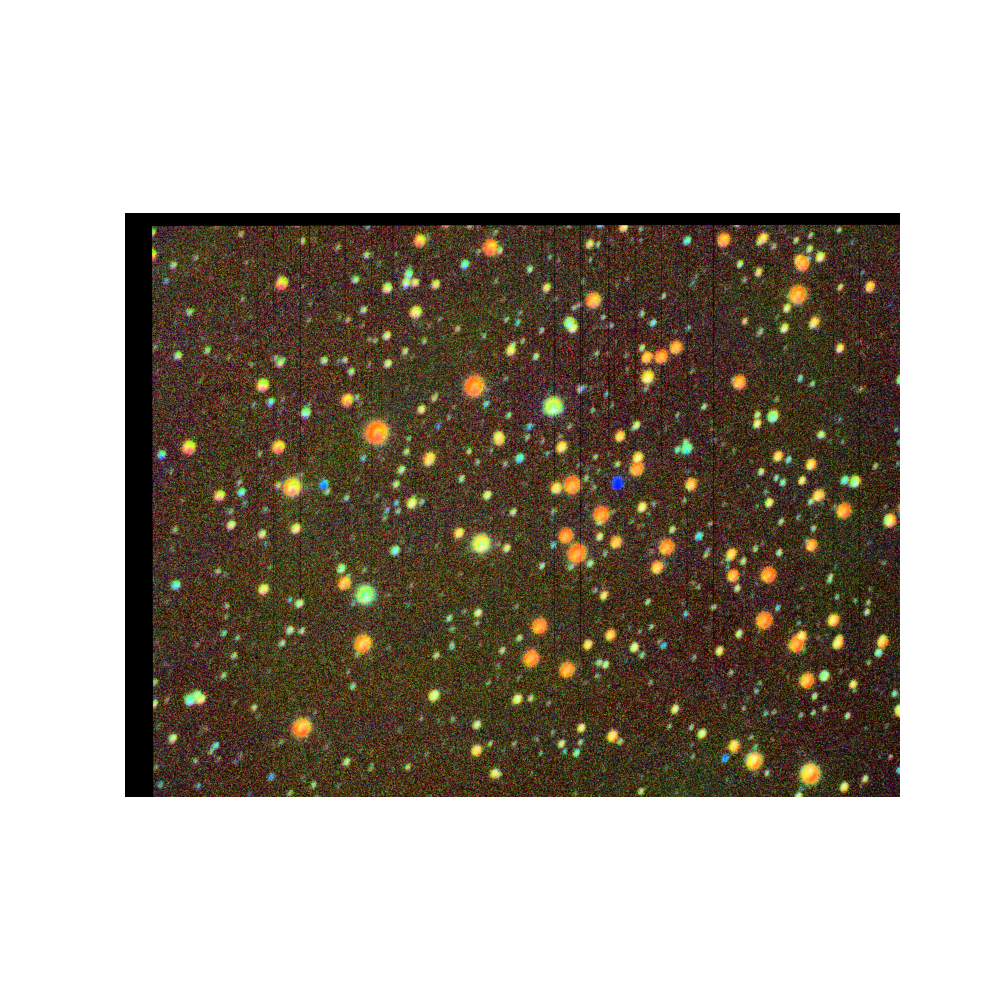
\includegraphics[width=0.9\linewidth]{ngc1528.png}
    \caption{NGC 1528 after cross matching of individual stars in g, r, i bands.}
    \label{fig:uncertainties}
\end{figure}

\subsection{Creation of Color-Magnitude Diagram}

The final step involved constructing a color-magnitude diagram (CMD) for the star cluster. The merged source catalog provided calibrated magnitudes in the g-, r-, and i-bands. The CMD was created by plotting (g - i) color on the x-axis and i-band magnitude on the y-axis. Isochrone models from the \texttt{uwastro465isos} package were overlaid on the CMD to estimate the cluster's age and metallicity. A grid search was performed over a range of ages and metallicities to minimize residuals between observed and model magnitudes, yielding best-fit parameters for the cluster. This is the python code used to generate the CMD:

\begin{lstlisting}[language=Python]
imag, g_i = merged_sources['gmag'] - merged_sources['imag'], merged_sources['imag']

models_with_residuals = []

for age in iso.get_list_of_ages():
    for z in iso.get_list_of_metallicities():
        model = iso.select_isochrone(age, z)
        model['g_i'] = model['gmag'] - model['imag']
        model = model.loc[model.label == 3]
        
        residuals = []
        for i_obs, g_i_obs in zip(imag, g_i):
            dist = np.sqrt((model['imag'] - i_obs)**2 + (model['g_i'] - g_i_obs)**2)
            closest_distance = np.min(dist)  
            residuals.append(closest_distance ** 2)

        residual_sum = np.sum(residuals)  

        models_with_residuals.append({'age': age, 'metallicity': z, 'residual_sum': residual_sum})

models_with_residuals.sort(key=lambda x: x['residual_sum'])
\end{lstlisting}

\begin{figure}[h]
    \centering
    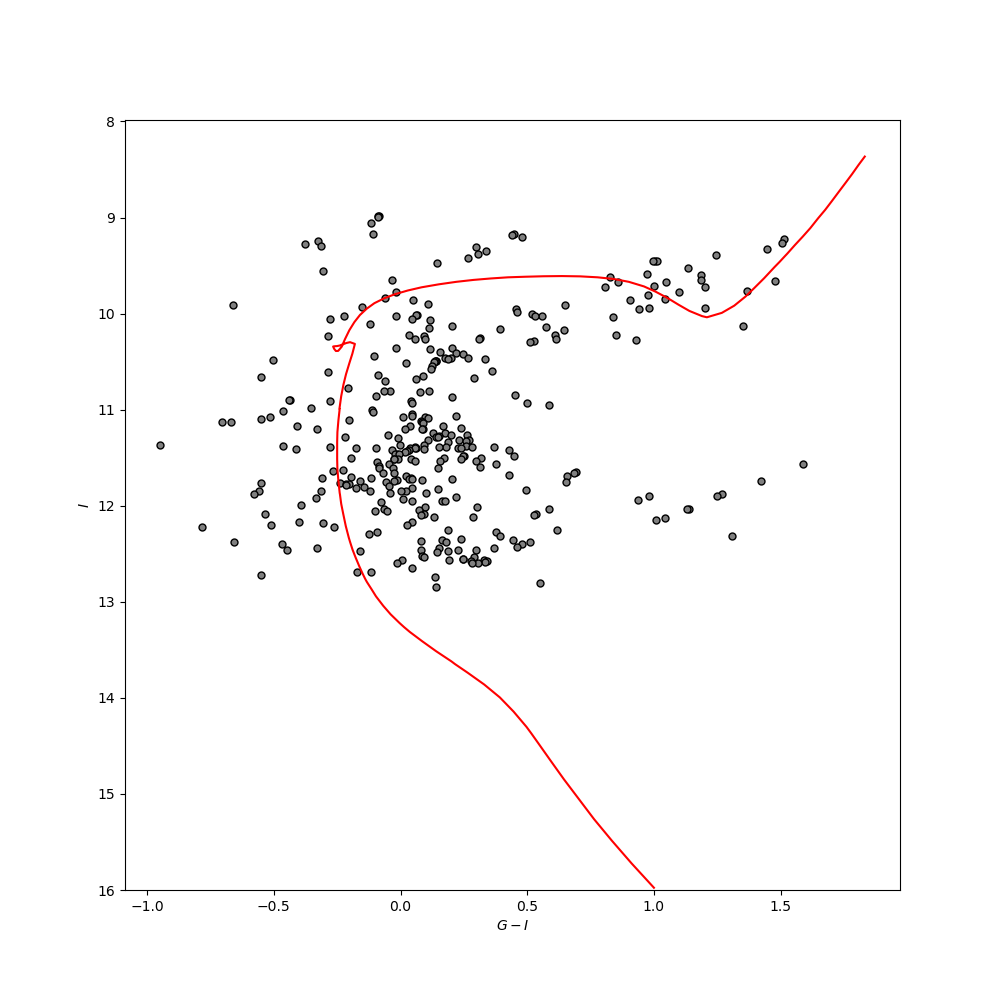
\includegraphics[width=0.9\linewidth]{cmd.png}
    \caption{The Color Magnitude Diagram of NGC 1528 with the theoretical isochrones to estimate the age of star cluster.}
    \label{fig:uncertainties}
\end{figure}

\subsection{Visualization and Summary}

Various visualizations were generated to summarize the analysis. These included scatter plots of signal-to-noise ratios for flux measurements, RGB composite image of the cluster field, and the final CMD with overlaid isochrones. The analysis demonstrated the effectiveness of the calibration and reduction pipeline, as well as the utility of multi-band photometry for characterizing star clusters. The detailed steps and results shows the importance of meticulous calibration and robust statistical methods in astronomical data analysis.

\section{Conclusions} \label{sec:conclusion}

The primary objective of this lab was to perform a photometric analysis of the star cluster NGC 1528 using CCD imaging and calibration techniques. Through a systematic approach to data collection, reduction, and analysis, the experiment successfully achieved the intended outcomes, providing valuable insights into the characteristics of the observed celestial objects.

\subsection{Calibration Process and Data Quality}

The use of master bias and master flat field frames significantly improved the quality and reliability of the science images. By mitigating electronic noise and correcting for pixel-to-pixel sensitivity variations, these calibration steps ensured the accuracy of the photometric measurements. The bias frames effectively captured the intrinsic electronic noise of the CCD detector, while the flat field images standardized the response of individual pixels. This calibration workflow enabled the reduction of systematic errors and provided a robust foundation for subsequent photometric analysis.

\subsection{Source Detection and Photometry}

The detection of astronomical sources within the science images was accomplished using the DAOStarFinder algorithm, which identified centroids of stellar objects and provided critical photometric properties such as flux and magnitude. By employing circular apertures for photometry and applying background subtraction, the analysis achieved reliable flux measurements for all detected sources. The resulting flux-to-noise ratio demonstrated consistency across the g, r, and i bands, with the g band exhibiting the highest signal-to-noise ratio due to its sensitivity to stellar emission in the green wavelength range.

\subsection{Color-Magnitude Diagram and Isochrone Fitting}

The creation of a color-magnitude diagram (CMD) for NGC 1528 served as a key analytical tool for understanding the stellar population of the cluster. By plotting the g-i color against the i-band magnitude, the CMD revealed the distribution of stars across different evolutionary stages. Isochrone fitting further refined the analysis, allowing the estimation of the cluster’s age and metallicity. The best-fit model indicated that NGC 1528 has an approximate age of 8.5 billion years and a metallicity consistent with solar abundance. The alignment of the isochrone with the observed data points validated the methodology and provided a detailed characterization of the cluster's stellar population.

\subsection{Astrometric Calibration and Catalog Matching}

The astrometric calibration of the science images ensured precise mapping of celestial coordinates, enabling comparisons with external catalogs such as Pan-STARRS. The matching process identified counterpart stars in the catalog and facilitated the calculation of photometric zero points for the g, r, and i bands. These zero points were critical for standardizing the observed magnitudes and integrating the data into a broader astrophysical context.

\subsection{Challenges and Limitations}

Despite the overall success, the lab encountered several challenges that influenced the data collection and analysis process. The telescope's initial tracking issues required careful adjustments to ensure accurate alignment and observation of the target field. Additionally, the faintness of certain stars in the i band introduced uncertainties in their photometric measurements. Future iterations of this experiment could benefit from extended exposure times and a larger sample of flat field and bias frames to further improve data quality.

\subsection{Final Remarks}

This lab demonstrated the importance of meticulous calibration, systematic analysis, and critical evaluation in astrophysical research. By combining advanced imaging techniques, computational tools, and theoretical models, the experiment provided a comprehensive understanding of the star cluster NGC 1528. The results not only highlight the significance of photometry in studying stellar populations but also underscore the potential for further investigations into the dynamics and evolution of star clusters.

\section{References}

\begin{enumerate}
    \item University of Wisconsin-Madison, \textit{Astronomy 465: Optical Astronomy Lab Manual}. University of Wisconsin-Madison, Department of Astronomy, 2024.
    
    \item University of Wisconsin-Madison, \textit{Astron 465 Lecture Slides}. University of Wisconsin-Madison, Department of Astronomy, 2024. Accessed during lectures.

    \item Howell, S. B. \textit{Handbook of CCD Astronomy}, 2nd edition. National Optical Astronomy Observatory and WIYN Observatory, 2006.

    \item University of Wisconsin-Madison, \textit{Sterling Rooftop Observatory Manual}. University of Wisconsin-Madison, Department of Astronomy, 2024.

    \item https://photutils.readthedocs.io/en/stable/index.html

\end{enumerate}

\end{document}
